\setlength{\arrayrulewidth}{0.5mm}
\setlength{\tabcolsep}{18pt}
\renewcommand{\arraystretch}{1.5}


\chapter{Marco Teórico} \label{cap:antecedentes}




Este capitulo se dedica a explorar y contextualizar los conceptos, tecnologías y metodologías esenciales que fundamentan la implementación del tablero de datos propuesto. \\

En este contexto, se abordarán conceptos clave como \texttt{PostgreSQL}, \texttt{Django}, y \texttt{ReactJS}, que desempeñan un papel fundamental en el diseño y funcionamiento de la aplicación. Además, hará una comparativa en diferentes bibliotecas y software para la visualización de datos, y el por qué se eligió el uso de la biblioteca \texttt{AmCharts} para la implementación del tablero.\\

El enfoque de este capítulo es proporcionar una comprensión  de las herramientas y tecnologías seleccionadas para el desarrollo del tablero de datos. Se profundizará en sus características, ventajas y casos de uso relevantes, estableciendo así una base sólida para la posterior discusión de la metodología y la construcción del tablero de datos.

\section{Base de datos}\label{sec:basedatos}
Las bases de datos son componentes esenciales en el ámbito de las Ciencias de la computación y más en especifico, en la creación de software. Proporcionan un mecanismo estructurado y eficiente para almacenar, organizar y recuperar datos de manera sistemática. \\
Más en concreto, en lo que concierne a las aplicaciones web, el uso de bases de datos permite gestionar grandes volúmenes de información de manera estructurada y accesible.

Existen diferentes tipos de bases de datos, y la elección del tipo adecuado depende de los requisitos específicos de la aplicación. \\

\subsection{Modelo relacional}
Hoy en día, el modelo de bases de datos más usado en todos los ámbitos, es el \textbf{relacional}. Este modelo se basa en la representación de datos en tablas, proporcionando una forma clara y estructurada de organizar la información. Cada tabla contiene registros que representan entidades únicas y columnas que almacenan atributos específicos de esos registros. La relación entre tablas se establece mediante claves únicas, permitiendo la conexión y consulta eficiente de datos.

\begin{figure}[h]
\centering
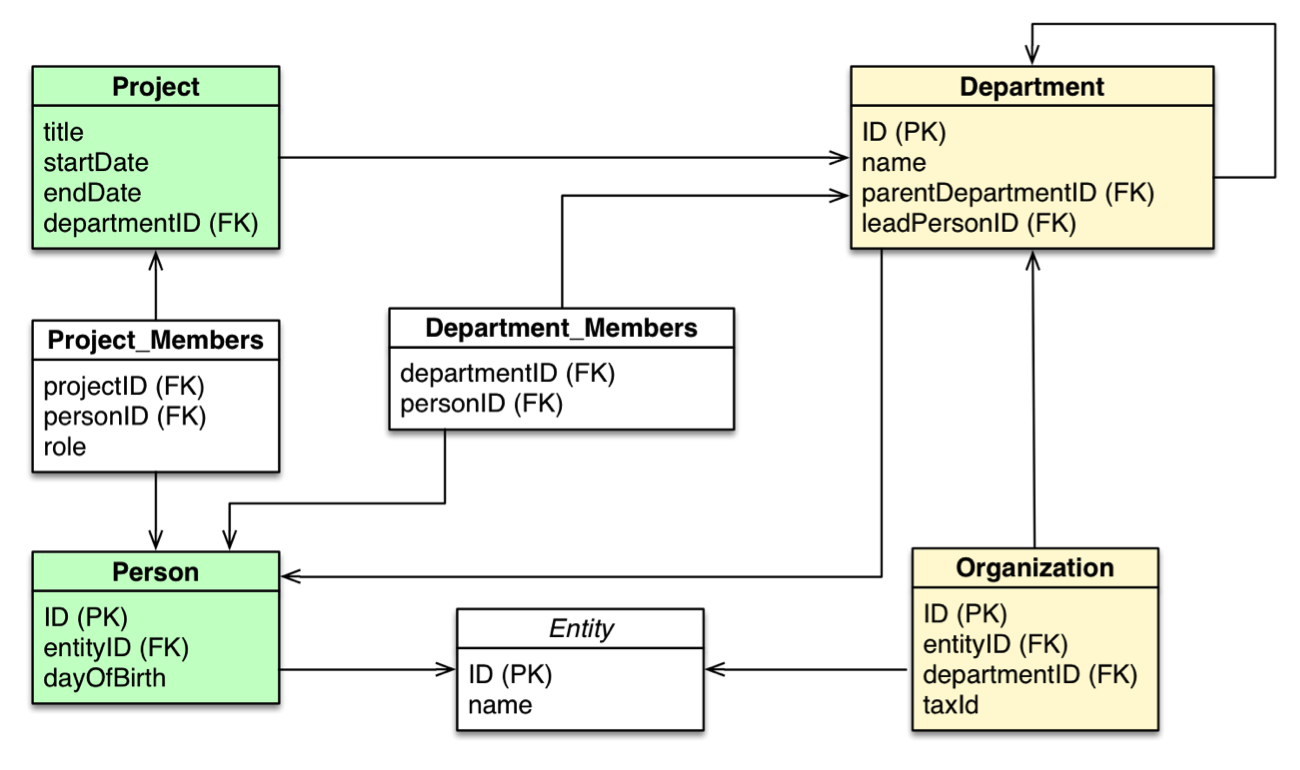
\includegraphics[width=0.5\textwidth]{images/ejemplo-modelo-relacional.png}
\caption{Ejemplo de un modelo relacional}
\end{figure}



Las bases de datos relacionales se basan en el modelo relacional, ya que este proporciona una forma estructurada de representar datos en tablas. \\En una base de datos relacional, cada fila de la tabla es un registro con un \textbf{\texttt{ID}} único denominado clave. Las columnas de la tabla contienen atributos de los datos, y cada registro suele tener un valor para cada atributo, lo que facilita establecer las relaciones entre los puntos de datos.\\


\subsection{Sistema de gestión de bases de datos}

Teniendo definido un modelo para implementar una base de datos, se debe tener un medio o herramienta con la cual interactuar para realizar operaciones como crear y borrar tablas, insertar y borrar datos, dar permisos de lectura y/o alteración, entre otro tipo de operaciones.\\
Para ejecutar este tipo de operaciones se utilizan los \textit{Sistema de gestión de bases de datos}. \\

Un \textbf{\textit{Sistema de gestión de bases de datos (DBMS, Data Base Management System)}} es un software que sirve como interfaz entre la base de datos y sus programas o usuarios finales, lo que permite a los usuarios recuperar, actualizar y gestionar cómo se organiza y se optimiza la información.\\ Un DBMS también facilita la supervisión y el control de las bases de datos, lo que permite una variedad de operaciones administrativas como la supervisión del rendimiento, el ajuste, la copia de seguridad y la recuperación.
\\
En esencia, este tipo de software actúa como un intermediario entre la aplicación y la base de datos, facilitando la interacción con los datos almacenados. A través de interfaces específicas, los usuarios pueden realizar diversas operaciones, asegurando la integridad y coherencia de la información contenida en la base de datos.\\

Por último, según el ranking de \textbf{DB-Engines}, a fecha de Enero del 2024\footnote{el ranking de DB-Engines se actualiza mensualmente.}, estos son los 10 mejores sistemas de gestión de bases de datos:

\begin{enumerate}
    \item Oracle
    \item MySQL
    \item Microsoft SQL Server
    \item PostgreSQL
    \item MongoDB
    \item Redis
    \item Elasticsearch
    \item IBM DB2
    \item Snowflake
    \item Microsoft Access
\end{enumerate}

\subsection{SQL (Structured Query Language)}

\texttt{SQL (Structured Query Language)} es un lenguaje declarativo de propósito especial
que se basa en conceptos del modelo relacional y el álgebra relacional que se utiliza en los sistemas de gestión de bases de datos relacionales. \texttt{SQL}, introducido a principios de los años 70, se utiliza hoy en día como componente básico de muchas aplicaciones de software y sigue siendo una herramienta fundamental y omnipresente para la manipulación de datos.\\

Además, hoy en día el poseer conocimientos avanzados en \texttt{SQL} no sólo es de utilidad para definir un modelo relacional e implementarlo en \textbf{DBMS}, sino que también se ha vuelto esencial en diversos ámbitos profesionales. \\
Cómo su nombre lo dice, \texttt{SQL} es un lenguaje que nos permite hacer consultas a bases de datos.\\
A través de \texttt{SQL}, es posible llevar a cabo una variedad de operaciones para obtener, insertar, actualizar y eliminar datos en una base de datos. \\
A continuación se muestran algunos tipos comunes de consultas que se pueden realizar con \texttt{SQL}:

\begin{enumerate}
    \item \textbf{Consulta básica (SELECT):}
    \begin{verbatim}
    SELECT columna1, columna2 FROM tabla;
    \end{verbatim}

    \item \textbf{Filtrado y ordenamiento de datos (WHERE, ORDER):}
    \begin{verbatim}
    SELECT * FROM empleados WHERE salario > 50000 ORDER BY apellido;
    \end{verbatim}

    \item \textbf{Operaciones de agregación (AVG, COUNT):}
    \begin{verbatim}
    SELECT AVG(edad), COUNT(*) FROM usuarios WHERE ciudad = 'Nueva York';
    \end{verbatim}

    \item \textbf{Unión de tablas (JOIN):}
    \begin{verbatim}
    SELECT clientes.nombre, pedidos.producto 
    FROM clientes INNER JOIN pedidos ON clientes.id = pedidos.cliente_id;
    \end{verbatim}

    \item \textbf{Inserción de datos (INSERT):}
    \begin{verbatim}
    INSERT INTO empleados (nombre, salario) VALUES ('Juan Perez', 60000);
    \end{verbatim}

    \item \textbf{Actualización de datos (UPDATE):}
    \begin{verbatim}
    UPDATE productos SET precio = precio * 1.1 WHERE categoria = 'Electrónicos';
    \end{verbatim}

    \item \textbf{Eliminación de datos (DELETE):}
    \begin{verbatim}
    DELETE FROM clientes WHERE fecha_registro < '2022-01-01';
    \end{verbatim}
\end{enumerate}


En el contexto empresarial, la habilidad para trabajar con bases de datos utilizando \texttt{SQL} se ha convertido en un requisito fundamental para roles en áreas como análisis de datos, ciencia de datos y desarrollo de software. La capacidad para extraer información valiosa, generar reportes y analizar grandes conjuntos de datos se ha vuelto crucial y cotidiano para la toma de decisiones informadas y estratégicas en las organizaciones, así como para reportar métricas y datos a las entidades gubernamentales.
\\
En lo que respecta al desarrollo de aplicaciones web, \texttt{SQL} se utiliza para la interacción con bases de datos donde se almacena y recupera información. Comprender cómo diseñar consultas eficientes y gestionar bases de datos de manera efectiva contribuye significativamente al rendimiento y la escalabilidad de las aplicaciones.\\

El conocimiento y manejo de \texttt{SQL} se ha convertido en un habilidad imprescindible en diversos sectores, y no se limita únicamente a la gestión de bases de datos. Su aplicación abarca desde la toma de decisiones estratégicas en el ámbito empresarial, el desarrollo eficiente de aplicaciones, hasta la exploración y análisis profundo de datos.


\subsection{PostgreSQL}

\texttt{PostgreSQL} es un sistema de gestión de base de datos objeto-relacional \textit{Open Source} que utiliza el lenguaje \textbf{SQL} combinado con muchas características que almacenan y escalan con seguridad las cargas de trabajo de datos más complicadas. \\
Los orígenes de \texttt{PostgreSQL} se remontan a 1986 como parte del proyecto \textbf{POSTGRES} de la Universidad de California en Berkeley y cuenta con más de 35 años de desarrollo activo en la plataforma central.\\

El uso de \texttt{PostgreSQL} puede ampliarse de amplias maneras, por ejemplo, añadiendo nuevos tipos de datos, funciones, operadores, funciones agregadas, métodos de índice, lenguajes procedurales y debido a la flexibilidad que permite, cada usuario puede utilizar cualquier propósito libre de cargo, modificar y distribuir \texttt{PostgreSQL}, no importa si uso es privado, comercial o académico.\\
Su flexibilidad incluye el poder trabajar con lenguajes procedurales como PL/pgSQL, Perl, Python y Tcl. También puede trabajar con otros lenguajes a través de extensiones como por ejemplo: Java, JavaScript (V8), R, Lua y Rust.\\
Esto hace de \texttt{PostgreSQL} una opción extremadamente versátil y adaptativa para una amplia gama de aplicaciones y escenarios de desarrollo.\\
Además, durante recientes años \texttt{PostgreSQL} se ha convertido en la base de datos relacional de \textit{Open Source} preferida por muchos desarrolladores empresariales y nuevas empresas, impulsando las principales aplicaciones empresariales y móviles, algunos ejemplos de su uso son:

\begin{itemize}
    \item Almacén de datos para soportar sus aplicaciones, soluciones y productos a escala de Internet.

    \item \texttt{PostgreSQL} admite objetos geográficos y puede utilizarse como almacén de datos geoespaciales para servicios basados en la localización y sistemas de información geográfica.

    \item Usado en el desarrollo de aplicaciones web y móviles.
\end{itemize}


\section{Frameworks de desarrollo web}\label{sec:framework}

Hoy en día, para el desarrollo y mantenimiento de aplicaciones web se hace uso de los \texttt{Frameworks de desarrollo web}.\\

Los \texttt{Frameworks de desarrollo web} son un tipo de software diseñado para facilitar el desarrollo de aplicaciones web al proporcionar medios que permiten a los desarrolladores enfocarse en las partes importantes del desarrollo. \\
Se encargan de facilitar tareas tediosas como el manejo de sesiones, la localización, la validación de entradas del usuario, formularios, herramientas para la visualización de datos, entre otras aplicaciones con una cantidad mínima de configuración. Esto hace que su uso sea práctico y reusable en el entorno de desarrollo web, ya que los desarrolladores no tienen que crear desde el inicio algunos de los componentes necesarios para un nuevo proyecto.\\

Por lo tanto, se puede decir que los propósitos principales para utilizar \textit{Frameworks} son:

\begin{itemize}
    \item Acelerar el proceso desarrollo.
    \item Reusar código existente.
    \item Promover buenas prácticas de desarrollo con el uso de patrones diseño.    
\end{itemize}

Actualmente existen diferentes \texttt{Frameworks de desarrollo web} disponibles en diferentes lenguajes de programación, sin embargo hoy en día los lenguajes más usado para el desarrollo de aplicaciones web son \textbf{JavaScript, Python} y \textbf{Java}. \\

JavaScript es ampliamente utilizado para el desarrollo del  Frontend, permitiendo la creación de interfaces interactivas y dinámicas en el navegador web. \\
Por otro lado, Python suele ser empleado tanto en el lado del Backend, como en el desarrollo de aplicaciones web completas a través de frameworks como Django y Flask. \\
Java también se mantiene como una opción popular, especialmente en grandes empresas.

\subsection{Backend}

El \texttt{Backend} se refiere a la parte de una aplicación web que no es visible para el usuario final, pero que es esencial para su funcionamiento. \\

Este se encarga de la configuración de todos los aspectos lógicos de la aplicación; engloba las funciones lógicas, de almacenamiento de datos y de seguridad necesarias para que la aplicación funcione de forma correcta y segura, de modo que todas las acciones solicitadas en la página web se ejecuten correctamente.
\\

Entre sus componentes que conforman el \texttt{Backend} de una aplicación web podemos encontrar los siguientes:

\begin{itemize}
    \item \textbf{Servidores}\\
     Se refiere a una máquina física o virtual que gestiona los recursos necesarios para ejecutar una aplicación web. Al recibir las peticiones de los usuarios, los servidores ejecutan la lógica necesaria y devuelven las respuestas a través de un protocolo de comunicación.

     \item \textbf{Lógica de la aplicación}\\
     Es la secuencia de operaciones que los desarrolladores programan en el \texttt{Backend} para realizar tareas.

     \item \textbf{Frameworks}\\
     Son bibliotecas para el \texttt{Backend} que los programadores utilizan para facilitar la escritura y actualización del código del servidor. Para el \texttt{Backend} existen bibliotecas de procesamiento de datos y herramientas que proporcionan acceso a segmentos de código funcionales.

    \item \textbf{Bases de datos}\\
    Contienen la información a la que acceden los servidores para completar las funciones directas de la aplicación y también tienen opciones para clasificar la información a la que pueden acceder diferentes usuarios.
\end{itemize}

Tener un \texttt{Backend} en una aplicación  web proporciona una base sólida para la gestión de datos, la seguridad, la escalabilidad y la eficiencia. También delimita claramente entre la lógica empresarial y la interfaz de usuario, agilizando tanto la gestión como el desarrollo a largo plazo de la aplicación.

\subsection{Django}
\texttt{Django} es un framework web de Python de alto nivel que fomenta el desarrollo rápido y el diseño limpio y pragmático, este framework se basa en el patron de diseño \textit{Modelo, Vista, Controlador (MVC)}.\\

%\begin{center}
    \begin{figure}[H]
        \centering
        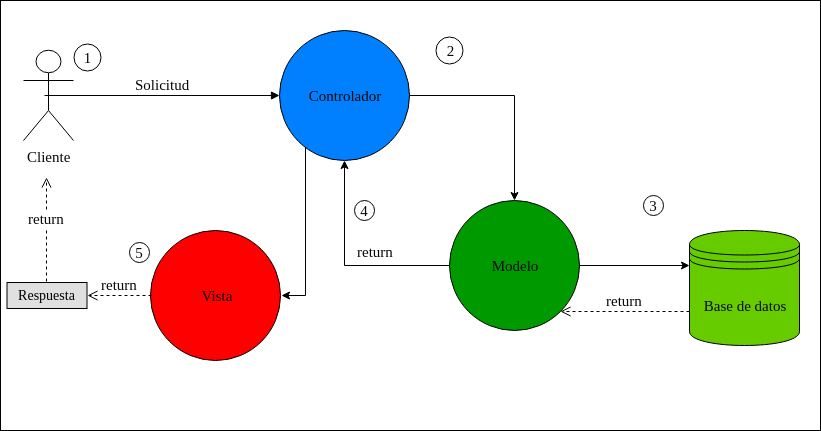
\includegraphics[width=0.7\textwidth]{images/MVC.png}
        \caption{Diagrama del funcionamiento del patrón de diseño \textit{MCV}}
    \end{figure}
%\end{center}


Hay amplias razones por las que hoy en día este framework web es elegido para desarrollar aplicaciones web, en concreto la parte correspondiente al \textbf{Backend}. Al explorar lo que ofrece, se puede observar que es extremadamente rápido y escalable, seguro y versátil, lo que lo convierte en una herramienta para el desarrollo rápido de aplicaciones web haciendo uso de código limpio y fácil de mantener.\\

Entre sus características, podemos encontrar las siguientes:
\begin{itemize}
    \item \textbf{Mapeador objeto-relacional (ORM, Object-Relational Mapper)}\\
    El ORM de Django permite a los desarrolladores interactuar con la base de datos usando código de Python, en lugar de escribir SQL en bruto. Esto hace que sea fácil trabajar con diferentes bases de datos y cambiar entre ellas si es necesario.

    \item \textbf{Interfaz de administración automática} \\
    Django proporciona una interfaz de administración incorporada que facilita la gestión de datos.
    
    \item \textbf{Sistema de plantillas}\\
    Django proporciona un dinámico sistema de plantillas que permite separar la representación de los datos de la lógica de la aplicación.

    \item \textbf{Enrutamiento URL}\\
    Django proporciona un eficaz sistema de enrutamiento de URLs que facilita la asignación de URLs a vistas.
    \\
\end{itemize}

Hablando en términos de escalabilidad, Django está probado y es escalable. Es utilizado por algunos sitios de tráfico pesado como Eventbrite, Disqus, Instagram, Prezi, Pinterest y Washington Post. Además, Django se puede acoplar con diferentes técnologias como \textit{ReactJS} para el libre desarrollo de los proyectos que hacen uso de este framerwork.

\subsection{Frotend}

En épocas pasadas, las páginas web se asemejaban a la estática disposición de las páginas de un libro, presentando información de manera fija y limitada. Este enfoque estático, sin embargo, distaba de satisfacer las expectativas de la experiencia moderna en la web.

Esencialmente, hoy en día una página web se compone de lenguaje de marcado de hipertexto (\textbf{HTML}), hojas de estilo en cascada (\textbf{CSS}) y \textbf{JavaScript}. El HTML define la estructura de una página web, el CSS estiliza la página, y JavaScript permite las interacciones del usuario. Los tres combinados se consideran desarrollo web \texttt{Front-end}.
Pero el desarrollo \texttt{Front-end} no sólo abarca el diseño y lógica de la aplicación. La responsividad y el rendimiento son los dos objetivos principales del \texttt{Front-end}. Un desarrollador debe asegurarse de que el sitio sea responsivo, es decir, que aparezca correctamente en dispositivos de todos los tamaños: ninguna parte del sitio web debe comportarse de forma anómala independientemente del tamaño de la pantalla.\\

Como se mencionó, \textbf{JavaScript} es el lenguaje encargado de las interacciones que los usuarios realicen; es un lenguaje de programación que los desarrolladores utilizan para hacer páginas web interactivas. Desde actualizar fuentes de redes sociales a mostrar animaciones y mapas interactivos, las funciones de JavaScript pueden mejorar la experiencia del usuario de una página web.\\
Adicionalmente, existen diversos Frameworks y bibliotecas para JavaScript que facilitan el desarrollo de aplicaciones web, algunos ejemplos son \textit{ReactJS}, \textit{AngularJS} y \textit{jQuery}.

\subsection{Visualización de datos}

El propósito principal de este trabajo es dar a conocer los datos obtenidos por SEDESA y mostrarlos en diferentes gráficas, pero el uso de gráficas no se limitaría únicamente a este módulo, también se usaría en diferentes módulos que quedan fuera del alcance de este trabajo. Para esto se debía hacer uso de gráficas de barras, barras empiladas, pastel, series de tiempo, mapas coropléticos y tablas.\\

Se exploraron diferentes bibliotecas de \textbf{JavaScript} que se podrían usar para la generación de gráficas. Se consideraron bibliotecas \textit{Open Source} y en las cuales se debían pagar una licencia por su uso.
La elección de la biblioteca para la visualización de datos no sólo se basó en sus capacidades técnicas, sino también en consideraciones de licencia. Se evaluaron las bibliotecas en términos de su adecuación para el proyecto, su compatibilidad con el flujo de trabajo y los requisitos de licencia asociados. Se buscó equilibrar la funcionalidad necesaria con la viabilidad económica y la alineación con los principios de código abierto cuando fuera posible.\\
En la Tabla 2.1 se presenta una comparativa de las bibliotecas de visualización de datos consideradas.\\

\begin{table}[ht]
    \centering
    \resizebox{\textwidth}{!}{%
        \begin{tabular}{ |p{2.5cm}|p{2.5cm}|p{4cm}|p{4cm}|  }
            \hline
            \textbf{Biblioteca} & \textbf{Software \textit{Open source}} & \textbf{Ventajas} & \textbf{Desventajas} \\
            \hline

            ChartJS & Sí & \begin{itemize}[left=0pt]
              \item Gráficas dinámicas y responsivas con un render de los valores previamente.
              \item Se maneja con canvas que da mejor rendimiento que SVG.
              \item Las gráficas se pueden descargar como imágenes.
              \item Se pueden configurar las gráficas.
              \item La curva de aprendizaje es sencilla.
            \end{itemize} & \begin{itemize}[left=0pt]
                \item Suele usarse para proyecto de menor escala.
            \end{itemize}. \\

            \hline
            D3 JS & Sí & \begin{itemize}[left=0pt]
                          \item Permite crear gráficos de vector.
                          \item Manejo de datos CSV, JSON y otros formatos.
                          \item Interacción con gráficos (zoom, desplazarse, arrastrar).
                          \item Manejo de datos geográficos.
                        \end{itemize} & \begin{itemize}[left=0pt]
                                            \item Se necesitan bibliotecas adicionales para exportar gráficos.
                                            \item La curva de aprendizaje es compleja.
                                          \end{itemize} \\
            \hline
            
            HighCharts & No & \begin{itemize}[left=0pt]
                                  \item Gran cantidad de gráficos dinámicos.
                                  \item Soporte técnico al obtener la licencia.
                                  \item Curva de aprendizaje intermedia por la gran documentación.
                                \end{itemize} & \begin{itemize}[left=0pt]
                                                    \item Para obtener todas las ventajas hay que pagar licencia.
                                                    \item Se cobra licencia por cada desarrollador que modificará la página.
                                                  \end{itemize} \\
            \hline
            
            AmCharts & No & \begin{itemize}[left=0pt]
                               \item Gráficas responsivas, interactivas y dinámicas.
                               \item La curva de aprendizaje es media.
                               \item Panel y modelos personalizables.
                             \end{itemize} & \begin{itemize}[left=0pt]
                                               \item Es libre para desarrollo, sin embargo se debe pagar licencia para integrarlo al proyecto.
                                             \end{itemize} \\
            \hline
        \end{tabular}%
    }
    \caption{Bibliotecas de visualización de datos}
\end{table}

Una vez hecho el análisis comparativo entre cada bibliotecas se llegaron a las siguientes conclusiones de acuerdo a cada biblioteca:

\begin{itemize}
    \item ChartJS es muy intuitivo de utilizar, responsivo y fácil de implementar, sin embargo, cuenta con gráficas básicas como líneas, barras y pie, pero dentro de los requerimientos surge la necesidad de utilizar mapas y aquí es donde carece esta biblioteca.

    \item D3JS tiene una amplia comunidad que le da soporte constantemente a los gráficos desarrollados en esta biblioteca, sin embargo, la curva de aprendizaje a utilizar es más amplia para el tiempo reducido que se cuenta para el proyecto. Su implementación requiere un cantidad líneas de código grande para una gráfica en apariencia sencilla, y su personalización es demasiado compleja.

    \item La biblioteca de HighCharts, además de estar enfocado en móviles y finanzas, también cuenta con características de navegación en altos volúmenes de información, anotaciones de usuarios y algunos indicadores técnicos, que si bien, harían que dichas gráficas tengo una mejor calidad en la presentación final, generan un aumento considerable en el costo final de la licencia, por lo que, al menos que se tenga la solvencia liberada para el proyecto, no sería de uso fundamental para el desarrollo de los tableros.

    \item AmCharts ofrece el mismo tipo de gráficas que HighCharts, siendo la gran diferencia el costo de la licencia y el hecho de qué al adquirir la licencia no existe un límite de desarrolladores que interactúen en la misma aplicación interna.
\end{itemize}








\subsection{AmCharts}

Después de juntas con representantes de \textbf{SEDESA} dónde expusieron las necesidades del proyecto en cuánto al tipo de gráficas que se necesitarían y comparándolo con las bibliotecas anteriormente mencionadas, se decidió optar por el uso de \texttt{AmCharts} en su versión 5.\\

Entre sus características más notorias se pueden mencionar las siguientes:

\begin{itemize}
    \item \textbf{Procesamiento de datos rápido}\\
    El procesamiento de datos dentro de \texttt{AmCharts 5} está diseñado para ser lo más eficiente posible. Las actualizaciones incrementales, la ausencia de agregaciones repetitivas y el uso de objetos de datos ligeros hacen que el procesamiento de datos sea rápido y eficiente en términos de memoria.

    \item \textbf{Plantilla de elementos}\\
    La mayoría de los elementos se crean utilizando plantillas: una colección de ajustes, eventos y adaptadores predeterminados. Al cambiar de plantilla, los cambios se propagan automáticamente a los elementos reales, lo que facilita las actualizaciones por lotes.

    \item \textbf{Estado de los elementos}\\
    La biblioteca permite cambiar fácilmente el aspecto de un elemento en diferentes circunstancias, por ejemplo, en alguna interacción, hover, clic, o en relación con los datos (por ejemplo, el aspecto de una columna si un valor está abajo).\\
    El motor aplicará automáticamente las propiedades requeridas según sea necesario, animando entre los valores antiguos y nuevos suavemente.
\end{itemize}

A partir del análisis realizado se puede decir que, \texttt{AmCharts 5 }es una robusta biblioteca de visualización de datos que ofrece un variado conjunto de opciones de visualización. \\
Admite gráficas tradicionales como líneas, áreas, columnas, dispersión, entre otras, con la flexibilidad de combinar estos tipos. También incluye gráficas porcentuales, circulares, de dona, mapas geográficos y visualizaciones especializadas como diagramas de Sankey, mapas de árbol, nubes de palabras y diagramas de Venn. Además, la biblioteca incluye funciones avanzadas como diagramas de Gantt, diagramas de cascada y visualizaciones de libro de pedidos/profundidad. Con opciones adicionales como diagramas de acordes, sunbursts e histogramas radiales, AmCharts 5 es una herramienta versátil para crear una amplia gama de visualizaciones de datos atractivas e informativas.



%-------------------------------------------------------------------
\section{Resumen}

%En este capítulo se expusieron la terminología y conceptos relacionados con ....



En este capítulo, se ha explorado y contextualizado la terminología y los conceptos fundamentales relacionados con la implementación del tablero de datos solictado. Se abordaron conceptos esenciales que abarcan desde la elección de la base de datos y su modelo relacional hasta la selección del sistema de gestión de bases de datos, haciendo hincapié en la importancia del lenguaje \texttt{SQL} en este contexto.\\

Además, se proporcionó una visión detallada de la elección de \texttt{PostgreSQL} como sistema de gestión de bases de datos, destacando su versatilidad y adaptabilidad. \\
Se discutió la relevancia de los frameworks de desarrollo web, centrándose en \texttt{Django} como una herramienta eficaz para el desarrollo del backend de aplicaciones web.
\\

La subsección dedicada a la visualización de datos examinó diversas bibliotecas de JavaScript, detallando sus ventajas y desventajas. Tras una exhaustiva comparación, se optó por el uso de \texttt{AmCharts 5} debido a su capacidad para generar gráficas dinámicas, responsivas e interactivas, además de su flexibilidad y versatilidad en términos de visualización de datos, costo y libertad para el uso dentro del equipo de trabajo.

En conclusión, este capitulo busca informar al lector de todas las tecnologías usadas para la implementación del tablero, se buscó dar a entender las diferencias, ventajas y desventajas de usar tecnologías \textit{Open source} como lo son \texttt{Django} y \texttt{PostgreSQL} en comparación con técnologias dónde se debe hacer la compra de la licencia para usarla como lo es \texttt{AmCharts}.